\section{Design Pattern utilizzati} \label{sec:designpatt}

\subsection{Dependency Injection}
\subsubsection{Descrizione}
Al fine di minimizzare le dipendenze delle classi implementate per il back-end del prodotto, è stato adottato il Dependency Injection pattern.\\
Lo scopo di questo pattern è separare il comportamento di una componente dalla risoluzione delle sue dipendenze, così da ridurne il grado di accoppiamento.
\subsubsection{Implementazione}
Nell'implementazione di questo pattern, è stata utilizzata Tsyringe, una libreria di Dependency Injection per Typescript. Attraverso l'utilizzo dei decoratori @injectable e @inject, è possibile dichiarare le classi le cui dipendenze sono iniettabili dal container e le singole dipendenze.\\
Una volta registrate questa dipendenze nel container, ed aver richiesto la 

\begin{figure}[h!]
    \centering  
    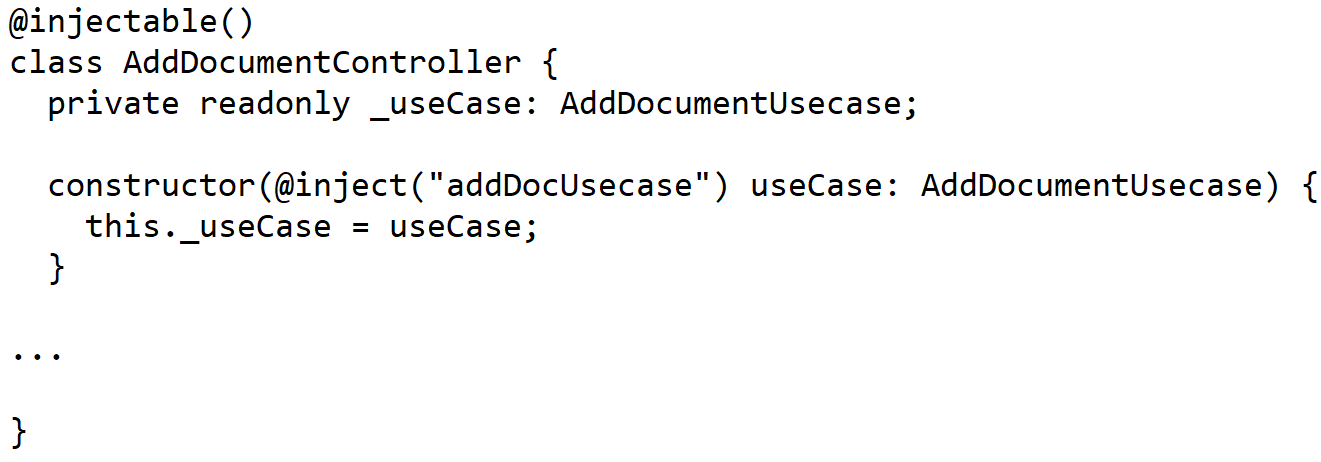
\includegraphics[width=0.7\textwidth]{DIinjectable.png}
    \caption{Esempio di implementazione nel prodotto di @injectable e @inject}
\end{figure}

\noindent Nell'esempio sopra riportato, "addDocUsecase" è il token associato alla classe dichiarata come dipendenza nel costruttore, e sarà utilizzato per registrare tale dipendenza nel container che si occuperà di iniettarla.\\
Una volta registrato, quando si chiederà di risolvere le dipendenze del controller, esse saranno risolte tramite Dependency Injection.

\begin{figure}[h!]
    \centering  
    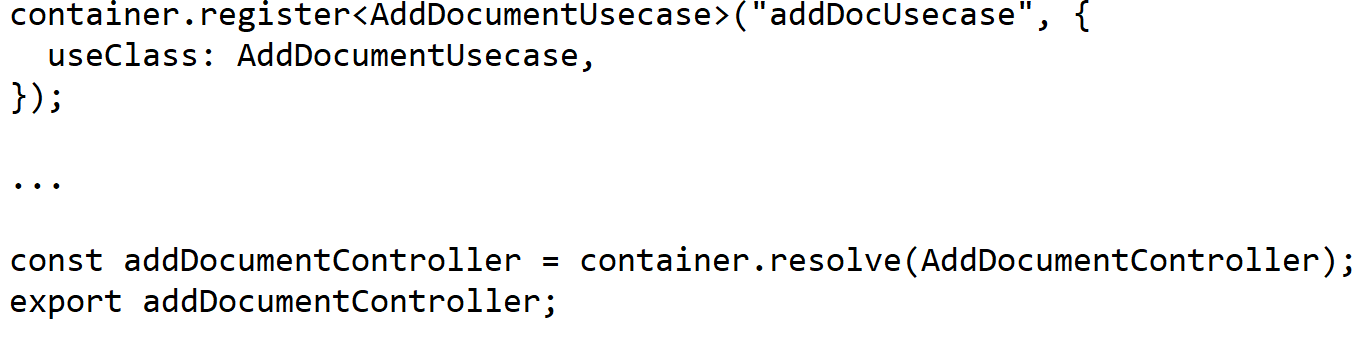
\includegraphics[width=0.7\textwidth]{DIcontainer.png}
    \caption{Esempio di registrazione e risoluzione delle dipendenze nel container Tsyringe}
\end{figure}

\newpage

\subsection{Controller-Service-Repository}
\subsubsection{Descrizione}
Coerentemente ai principi dell'architettura clean adottata per il sistema, per il back-end è stato utilizzato il CSR pattern. La business logic è implementata all'interno dei Service, che utilizzano i Repository per operare sui dati in lettura e scrittura. Adibiti ad elaborare le richieste e chiamare i Service, i Controller restituiscono i risultati delle operazioni al front-end.
\subsubsection{Implementazione}
Nell'implementazione di questo pattern, sono state definite delle classi Controller, Usecase e Repository.\\
Il Controller, come facilmente intuibile, riceve le richieste provenienti dal front-end, chiama lo Usecase associato e gestisce eventuali errori nell'esecuzione delle operazioni di business. Le classi Usecase rappresentano i Service, ovvero contengono la logica di business dell'applicazione, necessaria per l'esecuzione delle varie funzionalità. Ad essere chiamate dal Service sono le Repository, classi  responsabili della gestione della persistenza dei dati. Nascondono i dettagli della persistenza ai livelli superiori dell'applicazione, offrendo delle interfacce per recuperare e salvare i dati.
\\L'effettiva logica di accesso ai dati è delegata ai DataSource.

\newpage

\begin{figure}[h!]
    \centering  
    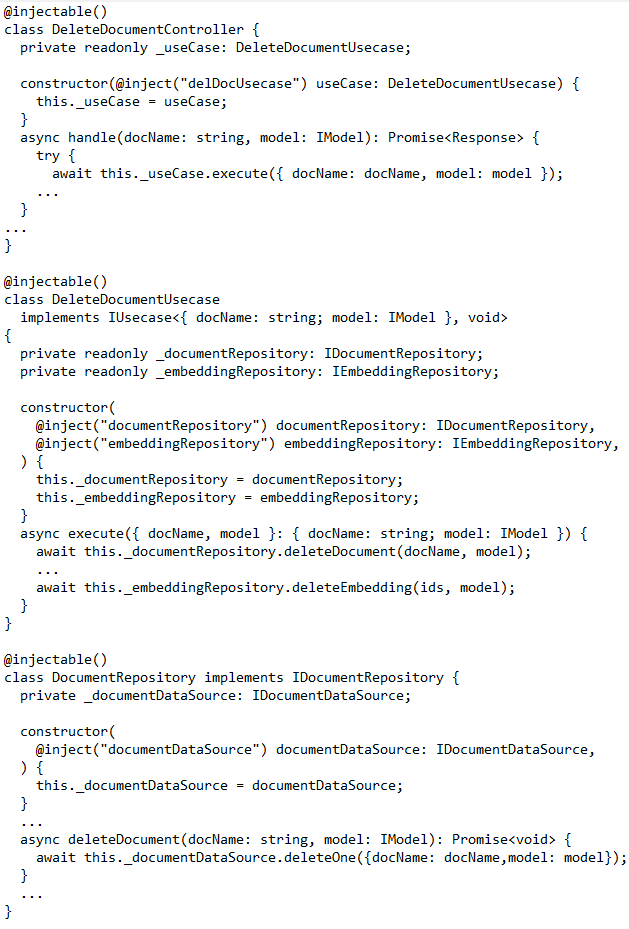
\includegraphics[width=0.75\textwidth]{CSR.png}
    \caption{Esempio di implementazione del CSR pattern per l'operazione di eliminazione di un documento}
\end{figure}

\newpage